\section{Model}

The TMD system is described by
the effective tight-biding, low-energy, two-valley Hamiltonian
\cite{PhysRevLett.108.196802},
\begin{equation}
H_{\tau}^{0}(\mathbf{k})=at\left(\tau k_{x}\hat{\sigma}_{x}+k_{y}\hat{\sigma}_{y}\right)+\frac{E_{g}}{2}\hat{\sigma}_{z}-E_{soc}\tau\frac{\hat{\sigma}_{z}-1}{2}\hat{s}_{z}\label{eq:H_tau_0}
\end{equation}
where the Pauli matrices $\hat{s}$'s operate in the spin space and
$\hat{\sigma}$'s operate in the orbital space with the two Bloch
orbital states $|v_{\tau s}^{\nu}(\mathbf{k})\rangle$ (indexed by
$\nu=+$ for the in-plane orbital state $|d_{x^{2}-y^{2}}\rangle+i\tau|d_{xy}\rangle$
and $\nu=-$ for the out-of-plane orbital state $|d_{z^{2}}\rangle$),
$s=\pm$ is the spin index, and $\tau=\pm$ is the valley index corresponding
to the $\pm\mathbf{K}$ point, respectively. The momentum $\mathbf{k}=\left(\begin{array}{cc}
k_{x}, & k_{y}\end{array}\right)$ is measured from the valley center. $a$ is the lattice constant
and $t$ is the hopping parameter. $E_{g}$ represents the energy
gap between the conduction and valence bands, and $2E_{soc}$ is the
spin splitting energy in the valence bands due to spin-orbit interaction.

The energy spectrum,
\begin{equation}
E_{\tau s}^{n}(k)=\frac{1}{2}\left(\tau sE_{soc}+n\sqrt{(2atk)^{2}+(E_{g}-\tau sE_{soc})^{2}}\right)\label{eq:energy}
\end{equation}
with $k = \abs{\vK}$
and $n = 1$ ($n = -1$) indexing the conduction (valence) band
is shown in \cref{fig:energy}.

\begin{figure}
  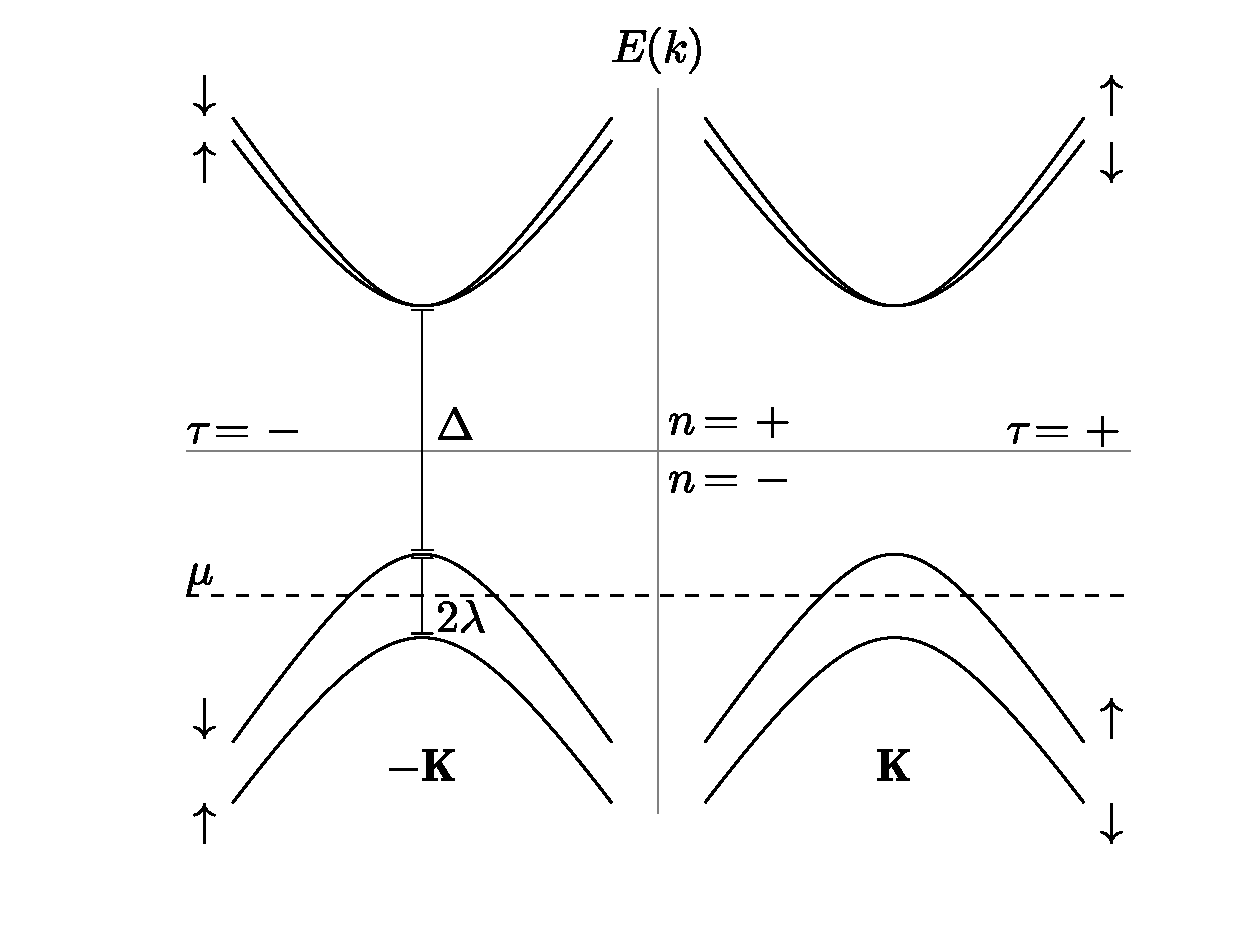
\includegraphics[width=\columnwidth]{figures/energy-bands}
  \caption{%
    Energy bands for $\ce{WSe2}$ as given by \cref{eq:energy}
    with $a t = \SI{3.939}{\electronvolt \per \angstrom}$,
    $E_g = \SI{1.60}{\electronvolt}$,
    and $E_{soc} = \SI{0.23}{\electronvolt}$.
    Each valley is centered at $± \vc{K}$ relative to the center of the
    Brillouin zone.
    The energy for a given band depends only on the distance $k$
    measured from the valley center.
  }\label{fig:energy}
\end{figure}

We focus on doped systems
such that the chemical potential $μ$ lies in the upper valence bands.
Within each band, the Bloch basis eigenstates are written
in terms of the orbital states as elements on the Block sphere,
\begin{equation}
  \begin{aligned}
    \Ket{u_{τ {\s}}^n \of{k, ϕ}}
    = & \cos{\frac{\fnTheta{n}}{2}} \ketOrb{+}{\of{k, ϕ}} \\
    + e^{-i τ ϕ}
      & \sin{\frac{\fnTheta{n}}{2}} \ketOrb{-}{\of{k, ϕ}},
  \end{aligned}
\end{equation}
where $k_x + i τ k_y = k e^{i τ ϕ}$ and
\begin{equation}
  \tan{\frac{\fnTheta{n}}{2}}
  = \frac{a t τ k}{\dfrac{E_g}{2} - \fnEnergy{-n} \of{k}}
  = \frac{a t τ k}{\fnEnergy{n} \of{k} - \fnEnergy{-} \of{0}}.
\end{equation}
The polar angle on the Bloch sphere
of the conduction and valence bands are related by
$\fnTheta{-} - \fnTheta{+} = τ π$.
The mapping of the energy band to the Bloch sphere,
parametrized by $\left( θ, ϕ \right)$,
encodes the topological character:
as one moves from the node out to infinity,
the states sweep either the northern or southern hemisphere
with a chirality determined by the Berry curvature.
